\subsection{Demand Calculation} \label{demandCalc}
%Janine

In Capitalism X, we assume that the demand for a product is based on customer satisfaction and the \textit{salesPrice}, the \textit{proxyPrice}, the \textit{totalProductQuality} and the \textit{proxyQuality}. 
The customer satisfaction influences the interest of the population in the respective products by shifting the price at which 100\% are interested.
 
The more satisfied customers are with the company, the more they are willing to pay for the same products. However, if customer satisfaction falls below 0.4, the \textit{overallAppeal} is influenced negatively. The following formula shows how the \textit{customerSatisfaction} affects the \textit{overallAppeal}.
\begin{equation}
\label{func:demandPrice}
\begin{aligned}
 oA_{demand} = 
\begin{cases}
    oA \cdot 1.2 & \text{if } cS \leq 0.8 \\
    oA \cdot 1.1 & \text{if } cS \geq 0.6 \\
    oA \cdot 1.05 & \text{if } cS \geq 0.5 \\
    oA \cdot 1 & \text{if } cS \geq 0.4 \\
    oA \cdot 0.9 & \text{if } cS \geq 0.2 \\
    oA \cdot 0.8 & \text{otherwise} \\
\end{cases}
\end{aligned}
\end{equation}

In order to make the demand of CapitalismX clients more similar to that of a real market, the demand curve is an S-shaped curve. This curve shows a larger slope at the beginning and end of the value range we use than in the middle.
\newline
The \textit{demandPercentage} (\gls{dPC}) is calculated by using the \textit{overallAppeal} as input for the following function. 
\begin{equation}
\label{func:demandPercentage}
\begin{aligned}
% 168*e^(-4.5*(10^-1)*(x^2))
dPC(oA_{demand}) = 168 \cdot e^{−4.5 \cdot 10^{ -1 } \cdot oA_{demand}^{ 2 } } \\
dPC = 
    \begin{cases}
        100\% & \text{if} \; dPC \geq 100\\
        0\% & \text{if} \; dPC \leq 0\\
    \end{cases}
\end{aligned}
\end{equation}

Figure FIGURE shows the course of the \textit{demandFunction}. The x-axis corresponds to the \textit{overallAppeal} of a product and the y-axis to the percentage interest of the population, the \textit{demandPercentage}. 

\begin{figure}
	\centering
	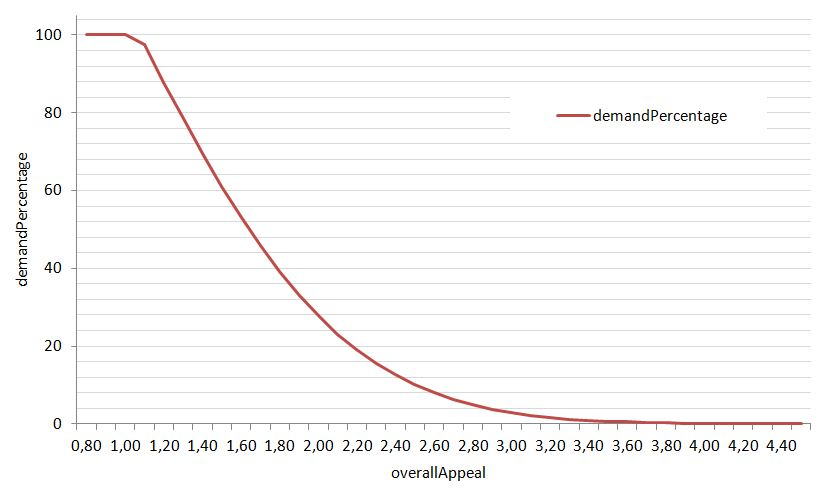
\includegraphics[width=12cm]{images/demand_function.JPG}
	\caption{Demand function}
	\label{jpg:demand_function}
\end{figure}

The \textit{totalDemand} (\gls{tD}) for a product is finally calculated by combining the demand in percent with the \textit{totalPopulation} (\gls{tP}). This approach enables the total demand to be higher than the actual quantity of products offered.
\begin{equation}
\label{func:totalDemand}
tD = dPC \cdot tP    
\end{equation}

The quantity actually sold by the company, so-called \textit{salesFigures} per product (\gls{sFP}), depends on whether the actual demand exceeds the \textit{numberOfferedProducts} (\gls{nOP}) or not.
\begin{equation}
\label{func:salesFigure}
\begin{aligned}
sFP = 
\begin{cases}
     nOP & \text{if} \; tD > nOP\\
     tD & \text{otherwise} \\
\end{cases}
\end{aligned}
\end{equation}

For the calculation of the \textit{marketShare} (\gls{mS}) it is assumed that the proportion of the population who would have liked to buy a product but went away empty-handed buys its product from a competitor. The company's \textit{totalMarketShare} (\gls{tMS}) is calculated using the sum of the sales figures of the single products and the sum of the demands for them. Following formulas show the calculation of the market share of a product and the total market share of the company.  
\begin{equation}
\label{func:marketShare}
\begin{aligned}
mS = \frac{sFP}{tD} \\
tMS = \frac{\sum(sFP)}{\sum(tD)}  
\end{aligned}
\end{equation}

